\documentclass[ngerman]{../LaTeX-Templates/Paper/paper}

\usepackage{nameref}
\usetikzlibrary{arrows,automata,positioning}


\title{Grundlagen der künstlichen Intelligenz}
\author{Simon König\\Skript und Zusammenfassung zur Vorlesung\\ von Marc \textsc{Toussaint}\\an der Universität Stuttgart}
\date{Stand \today}

\newcommand{\countset}[1]{\simpleset{1,\ldots,#1}}
\newcommand{\E}{\ensuremath{\operatorname{E}}}
\newcommand{\independent}{\ensuremath{\operatorname{Indep}}}
\newcommand{\enqo}[1]{\glqq #1\grqq\ }
\definecolor{green}{rgb}{0.2,0.8,0.2}
\lstset{ 
  backgroundcolor=\color{white},
  basicstyle=\footnotesize\ttfamily,
  breakatwhitespace=true,
  breaklines=true,
  captionpos=b,
  deletekeywords={},
  escapeinside={(*}{*)},
  mathescape=true,
  extendedchars=true,
  frame=lines,
  xleftmargin=10pt,
  keepspaces=true,
  keywordstyle=\bfseries\color{red!60!black},
  commentstyle=\itshape\color{gray!40!black},
  identifierstyle=\color{black},
  stringstyle=\color{green!40!black},      
  language=Java,
  morekeywords={*,...},
  numbers=left,
  numbersep=5pt,
  resetmargins=true,
  numberstyle=\tiny\color{gray!40!black},
  rulecolor=\color{black},
  showspaces=false,
  showstringspaces=false,
  showtabs=false,
  aboveskip=\medskipamount,
  belowskip=-2\medskipamount,
  stepnumber=1,
  tabsize=2,
  title=\lstname,
  emph=[1]{%Klassen o.ä.
	TreePolicy,
	RolloutPolicy,
	Backup
  },
  emphstyle=[1]{\scshape\color{blue!60!black}},
  emph=[2]{
  then,
  end
  },
  emphstyle=[2]{\bfseries\color{red!60!black}},
}




\begin{document}
\maketitle%
\tableofcontents

\section{Einführung}
\section{Banditen}
Wir wollen ein System analog zu einarmigen Banditen modellieren durch sogenannte \glqq Banditen\grqq. Wir sagen, es gibt $n$ mögliche Banditen zwischen denen man wählen kann, die zu treffende Entscheidung ist also einer der Banditen.

Jeder Bandit gibt einen Gewinn (\emph{reward}), der proportional zur Gewinnwahrscheinlichkeit des Banditen $y\sim P(y;\theta_i)$ ist. Hierbei sei der Parameter $\theta_i$ der Maschine unbekannt. Das Ziel ist es, den Gewinn über eine Menge von Zügen zu maximieren.

Dieses Entscheidungsmodell ist ein Archetyp für die verschiedensten Problemstellungen.

\begin{definition}\label{Banditenproblem}
	Sei $a_t\in\countset n$ die Entscheidung für einen Banditen zum Zeitpunkt $t$. Das zugehörige Ergebnis ist $y_t\in\R$. 

	Eine Strategie \emph{policy} verwendet das Wissen über alle bisher getroffenen Entscheidungen um einen nächsten Banditen auszuwählen
	\begin{equation*}
		\pi:[(a_1,y_1),(a_2,y_2),\ldots,(a_{t-1},y_{t-1})]\mapsto a_t.
	\end{equation*}
\end{definition}
Eine Problemstellung kann nun auf verschiedene Weisen definiert werden, so gibt es zwei grundlegende \emph{Ziel-Typen}. Man kann versuchen während des gesamten Zeitraums einen maximalen Gewinn zu erzielen. Das heißt Ziel ist es, ein $\pi$ zu finden, sodass der Gewinn insgesamt maximiert wird
\begin{equation}
	\max\left\langle\sum_{t=1}^Ty_t\right\rangle.\label{policy_exploit}
\end{equation}
Dieses Verhalten würde man als \emph{exploitation} bezeichnen.
Zum Beispiel könnte immer $a_t$ so gewählt werden, dass das maximale $y_t$ zu erwarten ist.

Auch möglich ist, zu fordern, dass nur die letzte Entscheidung die bestmögliche ist, das heißt
\begin{equation}
	\max\left\langle y_T\right\rangle,\label{policy_explore}
\end{equation}
was bedeutet, dass in den Schritten vor der letzten Entscheidung ohne Rücksicht auf die Rewards einer Entscheidung gelernt werden kann. Man setzt hier also den Fokus darauf zu \emph{explorieren} und alle Möglichkeiten auszuprobieren.
Man versucht mit der \emph{policy} aus \autoref{policy_explore} möglichst viel Wissen zu sammeln. Es wird auf exploration optimiert und versucht so die Unsicherheit über die Wahrscheinlichkeitsverteilung des Banditen zu minimieren.


Wissen über das System kann auf zwei Arten und Weisen dargestellt werden. Zum Einen durch den Verlauf der bisherigen Interaktion zwischen Agent und Banditen
\begin{equation*}
	h_t=[(a_1,y_1),(a_2,y_2),\ldots,(a_{t-1},y_{t-1})].
\end{equation*}
Aber auch eine Darstellung als Wahrscheinlichkeitsverteilung ist möglich. Der sogenannte \emph{belief state} ist
\begin{equation*}
	b_t(\theta)=P(\theta|h_t),
\end{equation*}
wobei $\theta=(\theta_1,\ldots,\theta_n)$ der Vektor der unbekannten Gewinnwahrscheinlichkeiten der einzelnden Banditen ist.




Wir betrachten im Folgenden einige Möglichkeiten Banditen nach einer Problemstellung zu bewerten und so Entscheidungen zu treffen.
\subsection{Upper Confidence Bound (UCB)}
Mit der \emph{upper confidence bound}-Methode versucht man einen guten Mittelweg zwischen exploitation und exploration zu gehen. 

Zunächst wählt man jeden Banditen (mindestens) einmal. Gute Entscheidungen kann man natürlich nur dann treffen, wenn zu jedem Banditen überhaupt Informationen bekannt sind. 

Das Ziel ist es, den Banditen zu wählen, der zum einen den höchsten Gewinn verspricht aber bei dem man zum anderen noch neue Informationen lernen kann.
Betrachtet man den Gewinn jedes Banditen als zufällig verteilte Variable, werden wir den Mittelwert schätzen und zukünftig versuchen die Unsicherheit über diese Schätzung zu verringern.

Sei also $n$ die Anzahl der Züge insgesamt, $n_i$ die Anzahl der Spielzüge und $\Delta_i$ die Summe der Gewinne, jeweils am Banditen $i$.

Wir schätzen den Mittelwert der Gewinne bisher als
\begin{equation*}
	\hat y_i=\frac{\Delta_i}{n_i}.
\end{equation*}
Für eine Konstante $\beta$ (meist $\beta=1$) wählen wir dann den Banditen $i$, der
\begin{equation*}
	\hat y_i+\beta \sqrt{\frac{2\ln n}{n_i}}
\end{equation*}
maximiert. 
Mit dieser Entscheidung bilden wir ein Konfidenzintervall um den tatsächlichen Mittelwert $y_i$, das heißt mit einer (relativ hohen) Wahrscheinlichkeit gilt
\begin{equation*}
	\hat y_i-\sigma_i<y_i<\hat y_i+\sigma_i.
\end{equation*}
Der Algorithmus wählt jeweils die obere Schranke als Vergleichswert der Banditen. Damit wird sowohl der geschätzte Gewinn als auch die Unsicherheit der Schätzung mit einbezogen.


\subsection{Monte Carlo Tree Search (MCTS)}
Die Monte Carlo-Simulation versucht mit einer großen Zahl an zufälligen Stichproben eine Verteilung $x_i\sim P(x)$ zu approximieren. Mit diesen Stichproben kann man eine Verteilung abschätzen. Zum Beispiel mit 
\begin{equation*}
	\langle f\rangle=\int_xP(x)f(x)\intd x\approx \frac1N\sum_{i=1}^Nf(x_i),
\end{equation*}
ein Integral.

Bei der \emph{Monte Carlo-Baumsuche (MCTS)} versucht man den erwarten Reward abhängig von einer gewählten Aktion $a$ zu schätzen. Genauer gesagt wird die $Q$-Funktion 
\begin{equation*}
	Q(s_0,a)=\E\set{\Delta}{s_0,a}
\end{equation*}
geschätzt, wobei der erwartete Reward durch ein Monte Carlo-Verfahren bestimmt wird. Das heißt man simuliert randomisiert viele \glqq Zukünfte\grqq\ und schätzt so den Reward abhängig von $a$. Das Simulieren einer Zukunft wird auch Rollout genannt.

Ein generisches MCTS-Verfahren sieht dann wie folgt aus.
\begin{lstlisting}
start tree V = {(*$v_0$*)}
while within budget do
	(*$v_l$*) := TreePolicy(V)
	append (*$v_l$*) to V
	(*$\Delta$*) := RolloutPolicy(V)
	Backup((*$v_l, \Delta$*))
end while
return best child of (*$v_0$*)
\end{lstlisting}

\begin{itemize}
	\item Mit der \textsc{TreePolicy}-Methode wird entschieden welcher Blattknoten expandiert wird. Der Rückgabewert ist also der vielversprechendste Knoten, abhängig von der Bewertungsfunktion.
	\item Die \textsc{RolloutPolicy} simuliert einen Rollout. Oft wird dies zufällig berechnet, mindestens jedoch randomisiert.
	\item \textsc{Backup} reicht den Reward vom Blattknoten zurück bis zur Wurzel durch. So kann im nächsten TreePolicy-Schritt von der Wurzel aus der beste Knoten ausgewählt werden. 
\end{itemize}
Man spricht von \emph{Flat Monte Carlo}, wenn die ausgerollten Zukünfte nicht gespeichert werden. Der Baum kann damit vergleichsweise flach gehalten werden. Entscheidend ist, dass das Baumwachstum - und damit der Speicheraufwand - mit diesem Verfahren auf vielversprechende Pfade fokussiert wird.

\paragraph{Upper Confidence Tree (UCT)}
Man kann auf das MCTS-Verfahren das bereits bekannte {\itshape Upper Confidence Bound}-System anwenden. Es handelt sich dabei dann um {\itshape Upper Confidence Tree (UCT)}.
\begin{itemize}
	\item Man wählt mithilfe von UCB den nächsten Knoten. Das heißt die \textsc{TreePolicy} wählt
	\begin{equation*}
		\underset{v'\in\partial(v)}\argmax\frac{Q(v')}{n(v')}+\beta\sqrt{\frac{2\ln n(v)}{n(v')}}
	\end{equation*}
	zum Expandieren.
	\item Die \textsc{Backup}-Methode aktualisiert alle Eltern $v$ von $v_l$ mit
	\begin{align*}
		n(v)&\leftarrow n(v)+1&&\text{Anzahl Rollouts}\\
		Q(v)&\leftarrow Q(v)+\Delta&&\text{Summe der Rewards.}
	\end{align*}
\end{itemize}


\section{Markov-Entscheidungsprozesse (MDP)}
Ein Markov-Entscheidungsprozess ist eine stochastische Formalisierung des Banditenproblems. Wir betrachten einen Agenten, der sich in einer Welt befindet. Das gesamte System befindet sich in einem Zustand $s$, der Agent kann Aktionen $a$ ausführen, die einen Zustandsübergang hevorrufen, er stellt also die Abbildung
\begin{equation*}
	(s_{0:t},a_{0:t},r_{0:t})\mapsto a_{t+1}
\end{equation*}
dar.
Der Agent erhält bei jeder ausgeführten Aktion einen Reward $r$.

\vspace{1em}
\noindent
\begin{center}
	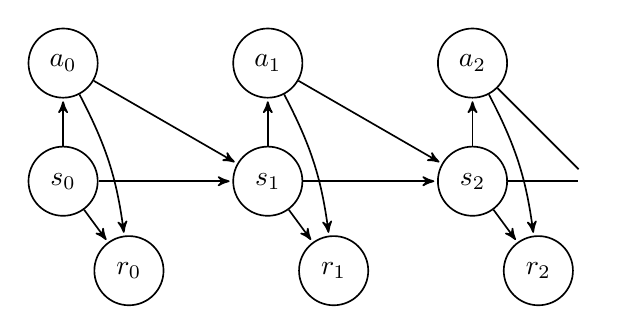
\begin{tikzpicture}[->,>=stealth',shorten >=1pt,auto,node distance=1.5cm,
                    semithick, baseline=1em]
	  \tikzstyle{every state}=[fill=white,draw=black,text=black]

	  \node[state] 		   (S0)                    	{$s_0$};
	  \node[state]         (S1) [right=1.7cm of S0] 		{$s_1$};
	  \node[state]         (S2) [right=1.7cm of S1] 		{$s_2$};

	  \node[state]         (A0) [above of=S0] 		{$a_0$};
	  \node[state]         (A1) [above of=S1]       {$a_1$};
	  \node[state]         (A2) [above of=S2]       {$a_2$};

	  \node[state]         (R0) [below right=0.5cm and 0.2cm of S0]	{$r_0$};
	  \node[state]         (R1) [below right=0.5cm and 0.2cm of S1]	{$r_1$};
	  \node[state]         (R2) [below right=0.5cm and 0.2cm of S2]	{$r_2$};

	  \node[]			(S3) [right of=S2] {};

	  \path (S0) edge (A0) edge (S1) edge (R0)
	  		(S1) edge (A1) edge (S2) edge (R1)
	  		(S2) edge (A2) edge[-] (S3) edge (R2)
	        (A0) edge[bend left=10] (R0) edge (S1)
	        (A1) edge[bend left=10] (R1) edge (S2)
	        (A2) edge[bend left=10] (R2)
	        (A2) edge[-] (S3);
	\end{tikzpicture}
\end{center}
\vspace{1em}

\noindent Da das gesamte System stochastischer Natur ist, lässt es sich mittels Wahrscheinlichkeitsverteilungen beschreiben. Es ist definiert durch
\begin{gather*}
	P(s_{0:T+1},a_{0:T},r_{0:T}; \pi)=\\P(s_0)\prod_{t=0}^TP(a_t|s_t;\pi)P(r_t|s_t,a_t)P(s_{t+1}|s_t,a_t).
\end{gather*}
Mit der initialen Zustandsverteilung $P(s_0)$, den Übergangsverteilungen $P(s_{t+1}|s_t,a_t)$, Verteilungen für den Reward $P(r_t|s_t,a_t)$ sowie der Policy des Agenten 
\begin{align*}
	\pi(a_t|s_t)&=P(a_0|s_0;\pi) &&\text{im stochastischen Fall, bzw.}\\
	a_t&=\pi(s_t)&&\text{deterministisch.}
\end{align*}%
In einem diskreten MDP können die Übergangswahrscheinlichkeiten $P(t_{t+1}|s_t,a_t)$ einfach als Tabelle gesehen werden.

Grundsätzlich wird angenommen, dass die Übergangs- und Rewardverteilungen unabgängig von der der Zeit sind und lediglich von Zustand und der getroffenen Aktion abhängen, diese Eigenschaft nennt man auch \emph{stationär}. 
Damit können wir die \emph{Rewardfunktion} sinnvoll definieren als
\begin{equation}\label{rewardfunction}
	R(s,a)\coloneqq\E\set{r}{s,a}=\int rP(r|s,a)\intd r.
\end{equation}

\paragraph{Zustandsbegriff in einem MDP}
Außerdem wichtig ist zu klären, was \enqo{Zustand} in einem MDP bedeutet. Wir definieren, dass für einen gegebenen Zustand die Vergangenheit konditional unabhängig von der Zukunft ist. Das heißt, alle möglichen \enqo{Zukünfte} $s_{t^+}$ für $t^+>t$ sind im Zustand $s_t$ kodiert. Oder allgemein
\begin{equation*}
	\forall t^+>t,t^-<t:\enspace\independent(s_{t^+},s_{t^-}|s_t).	
\end{equation*} 

\paragraph{Optimalität einer Policy}
Der \emph{Wert (Value)} eines Zustands $s$ beschreibt den erwarteten (discounted) reward bei einer Policy $\pi$, wenn in Zustand $s$ begonnen wird, das heißt
\begin{equation*}
 	V^\pi(s)\coloneqq\E\set{r_0+\gamma r_1+\gamma^2r_2+\ldots}{s_0=s;\pi}
 \end{equation*} 
mit Discounting-Faktor $\gamma\in[0,1]$. Das Discounting wird angewandt um Belohnungen in ferner Zukunft nur sehr klein zu bewerten.

Eine Policy $\pi^\ast$ ist optimal, wenn
\begin{equation*}
	\forall s:\enspace V^{\pi^\ast}(s)=V^\ast(s)\coloneqq\underset\pi\max\, V^\pi(s),
\end{equation*}
also gleichzeitig alle Values der möglichen Zustände maximiert werden.
In MDPs existiert immer mindestens eine optimale deterministische Policy.

\subsection{Valuefunktion}
Wir wollen noch einmal zurück zur Value-Funktion $V$ gehen und deren Eigenschaften betrachten. Sie ist ein zentrales Konzept in der gesamten Theorie des Reinforcement Lernens, denn viele Algorithmen lassen sich direkt aus ihr ableiten. Betrachten wir zunächst nur den Fall einer deterministischen Policy $\pi$, dann können wir die Valuefunktion rekursiv darstellen. Wir beginnen dazu mit der Definition
\begin{equation*}
	V^\pi(s)=\E\set{r_0+\gamma r_1+\gamma^2r_2+\ldots}{s_0=s;\pi}.
\end{equation*}
Den ersten Zustandsübergang und den damit einhergehenden Reward kann man nun herausziehen und erhält mit der Rewardfunktion aus \autoref{rewardfunction} dann
\begin{align*}
	V^\pi(s)&=\E\set{r_0}{s_0=s;\pi}\\
	&\quad+\gamma\E\set{r_1+\gamma r_2+\ldots}{s_0=s;\pi}\\
	&=R(s,\pi(s))\\
	&\quad+\gamma\sum_{s'}P(s'|s,\pi(s))\E\set{r_1+\ldots}{s_1=s';\pi}.
\end{align*}
Setzt man hier nun die Definition der Valuefunktion ein, erhält man die rekursive Darstellung
\begin{equation*}
	V^\pi(s)=R(s,\pi(s))+\gamma\sum_{s'}P(s'|s,\pi(s))V^\pi(s').
\end{equation*}
Der zweite Teil beschreibt den Wert/Value aller möglichen Folgezustände gewichtet mit den Wahrscheinlichkeiten der Übergänge.


Dies lässt sich genauso in Vektorschreibweise darstellen als
\begin{equation*}
	\mathbf V^\pi = \mathbf R^\pi+\gamma \mathbf P^\pi \mathbf V^\pi
\end{equation*}
mit den Vektoren $\mathbf V_s^\pi=V^\pi(s), \mathbf R_s^\pi=R(s,\pi(s))$ und der Wahrscheinlichkeitsmatrix $\mathbf P_{s,s'}^\pi=P(s'|s,\pi(s))$.

% \paragraph{Valuefunktion für stochastische Policies}
% Die rekursive Darstellung von $V$ für ein stochastisches $\pi(a|s)$ ist grundsätzlich analog
% \begin{equation*}
% 	V^\pi(s)=\sum_a\pi(a|s)R(s,a)+\gamma\sum_{s',a}\pi(a|s)P(s'|s,a)V^\pi(s').
% \end{equation*}

\subsubsection{Value Iteration}
Wir möchten nun einen ersten Ansatz finden, optimale Policies zu berechnen.
Wir verwenden dafür das Optimalitätsprinzip von Bellman, aus dem sich ergibt
\begin{equation*}
	V^\ast(s)=\max_a\bigg[R(s,a)+\gamma\sum_{s'}P(s'|s,a)V^\ast(s')\bigg].
\end{equation*}
Die zugehörige optimale Policy wählt immer die Aktion mit größtem erwarteten Reward, das heißt
\begin{equation*}
	\pi^\ast(s)=\underset a\argmax \bigg[R(s,a)+\gamma\sum_{s'}P(s'|s,a)V^\ast(s')\bigg].
\end{equation*}
Mit diesem Wissen lässt sich $V^\ast$ sinnvoll berechnen, das nachfolgende Verfahren ist die \emph{Value Iteration}.
Wir initialisieren $V_{k=0}(s)=0$. Dann berechnen wir für alle Zustände $s$ den Iterationsschritt
\begin{equation*}
	V_{k+1}(s)=\max_a\bigg[R(s,a)+\gamma\sum_{s'}P(s'|s,a)V_k(s')\bigg],
\end{equation*} 
bis das Abbruchkriterium
\begin{equation*}
	\max_s|V_{k+1}(s)<V_k(s)|\leq \epsilon
\end{equation*}
erreicht wird.


\subsection{Q-Funktion}
\subsubsection{Q-Iteration}

\begin{itemize}
	\item Q-Iteration und Q-Funktion 05/14ff
\end{itemize}





\subsection{Partiell beobachtbare Markov-Entscheidungsprozesse (POMDP)}
Partiell beobachtbare Markov-Entscheidungsprozesse (partially observable markov decision processes, POMDPs) sind MDPs
4/22ff
7/11ff

\paragraph{Anweden von MCTS auf POMDPs}

















\section{Reinforcement Learning}
Bisher sind wir davon ausgegangen, die Welt zu kennen. Genauer heißt das, dass $P(s'|s,a)$ und $R(s,a)$ bekannt waren. Damit konnten wir mittels Value- bzw. Q-Iteration (also mit dynamischem Programmieren) optimale Policies bestimmen.

Wenn diese Werte bzw. Verteilungen nicht bekannt sind, befindet man sich im Themengebiet des reinforcement Lernens.
Ein mit der Welt interagierender Agent sammelt den Datensatz
\begin{equation*}
	D=\simpleset{(s_t,a_t,r_t,s_{t+1})}_{t=1}^T
\end{equation*}
und versucht daraus zu lernen.

Man muss hierbei unterscheiden, ob ein Modell der Welt bekannt ist oder nicht. Das heißt, ob ein Agent alle möglichen Zustände und Aktionen erfassen kann oder nicht. Je nachdem ob man modellbasiert oder modellfrei lernt sind die Lernansätze unterschiedlich.
\noindent
\begin{center}
	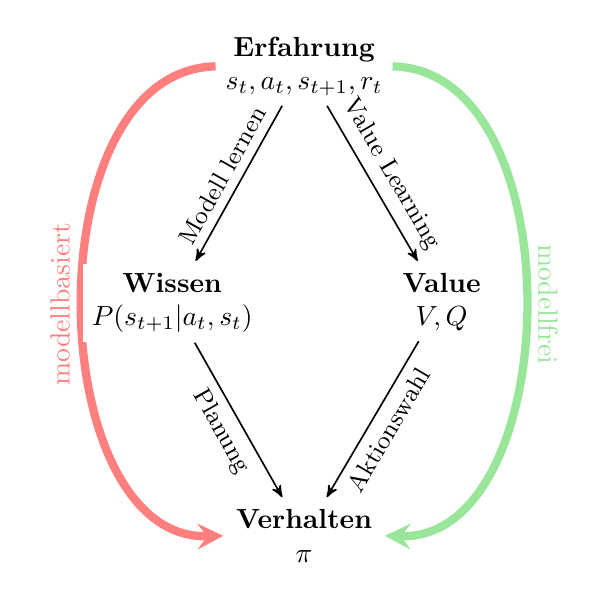
\begin{tikzpicture}[->,>=stealth',shorten >=1pt,auto,node distance=3.5cm,
                semithick, baseline=1em]
	  \tikzstyle{every state}=[fill=white,rectangle,draw=none,text=black,align=center]

	  \node[state] 		   (exp)                    	{\bf Erfahrung\\$\simpleset{s_t,a_t,s_{t+1},r_t}$};
	  \node[state]         (beh) [below=5cm of exp] 		{\bf Verhalten\\$\pi$};
	  
	  \begin{scope}[transparency group, opacity=0.5]
	  	\path (exp) edge[bend right=90,red,line width=3pt,-stealth] node[rotate=90,anchor=center,above]{modellbasiert} (beh);
	  	\path (exp) edge[bend left=90,green,line width=3pt,-stealth] node[rotate=-90,anchor=center,above]{modellfrei}(beh);
	  \end{scope}
	  


	  \node[state]         (kno) [below left=2cm and -0.6cm of exp] 		{\bf Wissen\\$P(s_{t+1}|a_t,s_t)$};
	  \node[state]         (val) [below right=2cm and 0cm of exp] 		{\bf Value\\$V,Q$};
	  

	  \path (exp) edge node[sloped, anchor=center, above]{\small Modell lernen} (kno) edge node[sloped, anchor=center, above]{\small Value Learning} (val)
	  (kno) edge node[sloped, anchor=center, below]{\small Planung} (beh)
	  (val) edge node[sloped, anchor=center, below]{\small Aktionswahl} (beh);
	  
	\end{tikzpicture}
\end{center}\noindent
Wir betrachten die genauen Unterschiede in den nachfolgenden Abschnitten.

\subsection{Modellfreies Reinforcement Learning}
Im modellfreien Reinforcement-Lernen sind die Übergangsverteilungen sowie die Rewards der Zustände unbekannt, es müssen nicht einmal alle Zustände bekannt werden. 
Ziel ist es zu lernen, den Value eines Zustands vorherzusagen. Das heißt die Algorithmen werden $V(s)$ bzw. $Q(s,a)$ schätzen.


\paragraph{On-Policy Off Policy Learning}



\subsubsection{Q-Learning}
Betrachten wir die Bellman-Optimalitätsgleichung für die $Q$-Funktion
\begin{equation*}
	Q^\ast(s,a)=R(s,a)+\gamma\sum_{s'}P(s'\,|\, s,a)\max_{a'}Q^\ast(s',a').
\end{equation*}
Wir möchten wieder basierend auf dieser Gleichung einen Algorithmus entwickeln der genauso wie die Q-Iteration ein $Q^\ast$ approximiert.
Doch ohne Modell der Welt kennen wir den zweiten Teil der Formel nicht, weder die möglichen Aktionen $a'$ noch die möglichen Zustände $s'$ sind bekannt.

Stattdessen lernen wir aus einzelnen Erfahrungen $(s,a,r,s')$ um so die $Q$-Funktion zu schätzen. Für jede Erfahrung berechnen wir basierend auf der vorherigen Q-Funktion die neue Approximation
\begin{align*}
	Q_{\text{new}}(s,a)&=(1-\alpha)Q_{\text{old}}(s,a)\\
	&\quad+\alpha[r+\gamma\max_{a'}Q_{\text{old}}(s',a')],
	\intertext{was wir weiter umformen zu}
	Q_{\text{new}}(s,a)&=Q_{\text{old}}(s,a)\\
	&\quad+\alpha\underbrace{[r+\gamma\max_{a'}Q_{\text{old}}(s',a')-Q_{\text{old}}(s,a)]}_{\text{TD error}}.
\end{align*}
So wird mit jedem Schritt der sogenannte \emph{temporal difference error} berechnet und als Korrekturfaktor addiert.
Ist der Reward $r$ größer als der erwartete Reward, das heißt
\begin{equation*}
	r>Q_{\text{old}}(s,a)-\gamma \max_{a'}Q_{\text{old}}(s',a'),
\end{equation*}
dann wird $Q_{\text{new}}(s,a)$ erhöht. Analog wird der Wert verringert, wenn $r$ kleiner als die Erwartung ist.
Dieses Verfahren wird \emph{Q-Learning} genannt.

Besonders bemerkenswert ist, dass eine mit Q-Learning gelernte Q-Funktion beweisbar gegen $Q^\ast$ konvergiert. Für den Beweis wurde lediglich die \emph{mixing property} angenommen. Das heißt, dass es von jedem Zustand aus eine Wahrscheinlichkeit $>0$ gibt in jeden anderen Zustand zu gelangen.

Ein Pseudocode des Q-Learning-Algorithmus sieht dann wie folgt aus.
\begin{lstlisting}
(*$Q(s,a)=0$*)
while unhappy
	initialize start state (*$s$*)
	while in episode
		Choose action (*$a\approx_\epsilon\underset a\argmax Q(s,a)$*)
		Take action (*$a$*), observe (*$r,s'$*)
		(*$Q(s,a)\leftarrow Q(s,a)+\alpha[r+\gamma\max_{a'}Q(s',a')-Q(s,a)]$*)
		(*$s\leftarrow s'$*)
	end
end\end{lstlisting}
Hierbei wurde die sogenannte \emph{epsilon greedy}-Strategie ($\approx_\epsilon$) verwendet. Das bedeutet lediglich, dass mit Wahrscheinlichkeit $\epsilon$ eine zufällige Aktion gewählt wird und nur mit Wahrscheinlichkeit $1-\epsilon$ tatsächlich das gewünschte $\argmax$. In Formel also
\begin{gather*}
	a\approx_\epsilon \underset a\argmax Q(s,a)\Longleftrightarrow\\ a=\begin{cases}
		\text{random},&\text{Wahrscheinlichkeit }\epsilon\\
		\underset a\argmax Q(s,a),&\text{sonst.}
	\end{cases}
\end{gather*}
Damit wird sichergestellt, dass der Algorithmus genügend exploriert und neue Daten sammelt, also eben nicht immer die optimale Aktion ausführt. Somit werden zum Beispiel lokale Maxima vermieden.

Desweiteren wird der Algorithmus in sogenannten Episoden ausgeführt, nach denen jedes mal der Startzustand wiederhergestellt wird bevor der Agent weiter agieren kann. Oft ist die Anzahl der auszuführenden Schritte in einer Episode festgelegt. Episoden stellen sicher, dass der Agent nicht in non-return areas gefangen bleibt und Lernen für immer verhindert wird (Klippe heruntergefallen, Objekt mit dem interagiert wird ist kaputt,\ldots).

\subsubsection{Varianten des Q-Learning}
06/15ff
\paragraph{Eligibility Traces}
\begin{itemize}
	\item Eligibility Traces
	\item Experience Replay
\end{itemize}
\paragraph{TD}
\paragraph{SARSA}
\paragraph{Q(lambda)}






\subsection{Modellbasiertes Reinforcement Learning}
06/23ff




Im modellbasierten Reinforcement Learning 

Der Agent wird dann versuchen
\begin{itemize}
	\item den nächsten Zustand vorherzusagen, genauer $P(s'|s,a)$ und
	\item den zugehörigen Reward, also $P(r|s,a)$ zu schätzen.
\end{itemize}








\begin{align}\label{Bellman1}
	V^\ast(s)&=\max_aQ^\ast(s,a)\\
	&=\max_a\left[R(s,a)+\gamma\sum_{s'}P(S'\,|\, s,a)V^\ast(s')\right]\nonumber
\end{align}


\begin{align}\label{Bellman2}
	Q^\ast(s,a)=R(s,a)+\gamma\sum_{s'}P(s'\,|\,s,a)\max_{a'}Q^\ast (s',a')
\end{align}

\begin{itemize}
	\item State-Action Value Funktion, Q
	\item Q-Iteration
	\item Belief State
	\item Lernen in MDPs, modellbasiert/modellfrei
	\item Diskussion Grenzen von modellfreiem Lernen 
	\item R-MAX
\end{itemize}




\subsection{Q-learning} Folie 11/50



Aus den neuen Erfahrungen die Zustände und Aktionen zu bewerten ist Reinforcement Learning

Schätzen und mit Lernrate $\alpha$ langsam annähern. Ohne Lernrate ist der Teil nach $\alpha$ zu stochastisch verrauscht. Neue Schätzung mit Low-Pass-Filter versehen. Lernen aus einer einzigen Erfahrung.

R(s,a): Erwartungswert der sofortigen Belohnung wenn ich Aktion a in Zustand s ausführe

Q-Funktion: Wie viel 

V-Funktion: $V^\pi(s)$ Return den ich erwarte wenn ich Policy $\pi$ benutze. $V^\ast$ optimales Verhalten










\section{Constraint Satisfaction Problems}
Constraints Statisfaction Probleme sind häufige auftretende Probleme


\begin{definition}[Constraint Satisfaction Problem]
	Ein \emph{Constraint Satisfaction Problem (CSP)} ist besteht aus $n$ Variablen $x_i$ mit zugehörigen \emph{Domains} $D_i, x_i\in D_i$ und $K$ \emph{Constraints} $C_k$.
	Jedes Constraint trifft eine Aussage über die Belegung einer Teilmenge aller Constraints. Genauer ist ein Constraint $C_k$ ein Tupel $C_k=(I_k,c_k)$ wobei $I_k\subseteq\simpleset{1,\ldots,n}$ die Teilmenge der betroffenen Variablen ist. Die Abbildung $c_k:D_k\rightarrow \simpleset{0,1}$ bestimmt, ob die Konfiguration der $c_{I_k}\in D_{I_k}$ zulässig ist.

	Das Ziel ist, eine Konfiguration $X=(X_1,\ldots,X_n)$ aller Variablen zu finden, sodass alle Constraints erfüllt sind.
\end{definition}


Ein CSP lässt sich als \emph{Constraint Graph} darstellen. Dies ist ein bipartiter Graph, in dem Variablen als Kreise und Constraints als Kästen dargestellt werden.

Betrachten wir das folgende Beispiel

\noindent
\vspace{1em}
\begin{center}
	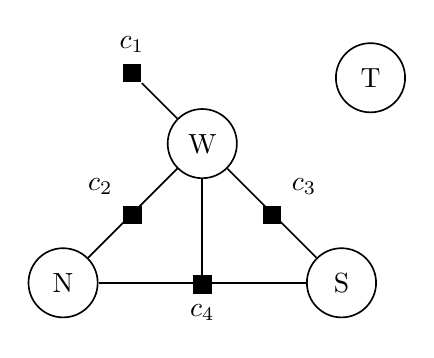
\begin{tikzpicture}[auto,node distance=2.5cm,semithick, baseline=1em]
	  \tikzstyle{every state}=[fill=white,circle,draw=black,text=black,align=center]

	  \node[state] (W) {W};
	  \node[state] (N) [below left of=W] {N};
	  \node[state] (S) [below right of=W] {S};
	  \node[state] (T) [above right=0.2cm and 1.5cm of W] {T};

	  \path (W) edge node[rectangle, fill=black, label={above left:$c_2$},below=-3pt]{} (N)
	  (N) edge node[rectangle, fill=black, label={below:$c_4$},below=-3pt]{} (S)
	  (W) edge node[rectangle, fill=black, label={above right:$c_3$},below=-3pt]{} (S)
	  node[rectangle, fill=black, label={above:$c_1$},above left=0.45cm and 0.45cm of W]{} edge (W)
	  node[below=1.4cm of W] {} edge (W);
	\end{tikzpicture}
\end{center}
\noindent
Dieses CSP hat 4 Variablen und ebenfalls 4 Constaints. Man sieht, dass die Constraints unterschiedliche Anzahlen an Variablen beeinflussen können.
Es gilt $I_1=\simpleset{W},I_2=\simpleset{W,N},I_3=\simpleset{W,S}$ und $I_4=\simpleset{N,W,S}$. Auch möglich ist, dass eine Variable von keinem Constraint beeinflusst wird, wie an $T$ zu sehen.
\begin{itemize}
	\item $C_1$ ist ein sogenanntes \emph{unäres Constraint}, da $|I_1|=1$.
	Ein Beispiel wäre $T\neq \text{rot}$.
	\item Die Constraints $C_2,C_3$ sind \emph{binäre Constraints}, da $|I_2|=|I_3|=2$. Ein Beispiel wäre $W\neq N$.
	\item Und das Constraint $I_4$ ist ein Constraint \emph{höherer Ordnung}, da $|I_4|>2$.
\end{itemize}

\subsection{Inferenz}



\begin{itemize}
	\item Inferenz
	\item Constraintgraphen
	\item Lösungsmethoden/Algorithmen: zunächst einfaches Backtracking, dann mit Heuristiken + Constraint Propagation + Arc Consistency/Propagation
	\item 
\end{itemize}



\section{Graphische Modelle von probabilistischen Problemen}
\begin{itemize}
	\item Bayesnetze
	\item Konditionale Unabhängigkeit
	\item 
\end{itemize}

\section{Inferenz in graphischen Modellen}
\begin{itemize}
	\item Variablenelimination
	\item Faktorgraphen
	\item Message Passing
	\item Loopy belief propagation
	\item Sampling Methods?
\end{itemize}


\section{Dynamische Modelle}
\begin{itemize}
	\item Markov Prozesse
	\item Hidden Markov Models
\end{itemize}


\section{Neuronale Netze}
\subsection{Graphische Repräsentationen}


\section{Erklärbarkeit von Entscheidungen}







\section{unassigned}
\begin{itemize}
	\item Belief Space Planning for Bandits 07/22ff
\end{itemize}
\end{document}
